\documentclass[10pt]{article}

\usepackage{answers}
\usepackage{setspace}
\usepackage{graphicx}
\usepackage{enumitem}
\usepackage{multicol}
\usepackage{circuitikz}
\usepackage{adjustbox}
\usepackage{mathrsfs}
\usepackage{mathtools}
\usepackage{fancyhdr}
\usepackage{svg}
\usepackage[margin=1in]{geometry}
\usepackage{amsmath,amsthm,amssymb}
\usepackage[compact]{titlesec}
\titlespacing{\section}{0pt}{*0}{-10pt}
\titlespacing{\subsection}{0pt}{*0}{-10pt}
\titlespacing{\subsubsection}{0pt}{0pt}{-10pt}
\parindent 0in
\parskip 12pt
\setlength{\headsep}{-10pt}
\setlength{\topskip}{0pt}
\setlength{\topmargin}{0pt}
\setlength{\topsep}{0pt}
\setlength{\partopsep}{0pt}
\geometry{margin=1in, headsep=0.25in}
\setlist[itemize]{label={--}, topsep=-10pt, noitemsep}
\setlist[enumerate]{topsep=-10pt, noitemsep}
\newcommand{\N}{\mathbb{N}}
\newcommand{\Z}{\mathbb{Z}}
\newcommand{\C}{\mathbb{C}}
\newcommand{\R}{\mathbb{R}}


\pagestyle{fancy}
\lhead{Aditya Arora}
\rhead{page \thepage}
\cfoot{ECE 222 Digital Computers}
\renewcommand{\headrulewidth}{0.2pt}
\begin{document}
\section*{Pipelining}
Pipelining is one architectural technique for improving speed
of programs. Multiple stages of different instructions are executed in different sections of the processor i.e. overlapped execution of instructions. \textit{note that it improves throughput and not latency}\\
An easier way to think of it is an assembly line of a car, with a new car rolling out once every few seconds but each car taking days.
\subsubsection{Hazards}
Although the throughput is improved generally, there are often cases where the pipeline must stall.
\begin{itemize}
    \item Data Dependency: The computation of Instruction i, depends on the computation result of an instruction further ahead in the pipeline [\textit{data hazard} specifically Read-after Write [\textit{RAW}]]
    \item Memory Delay: Memory takes too long to read or write (i.e. MFC takes a while to assert)
    \item Branch conditions: We realize the condition is a branch, so must discard any computation of the instructions right after the branch
\end{itemize}
\textit{Hazard}: Any condition that causes the pipeline to stall is called a hazard
How to get rid of data hazards:
\begin{enumerate}
    \item Stall: Stall the pipeline, by forcing a NOP [no operation \textit{bubble}] on each of the instruction ahead in the pipeline\\
    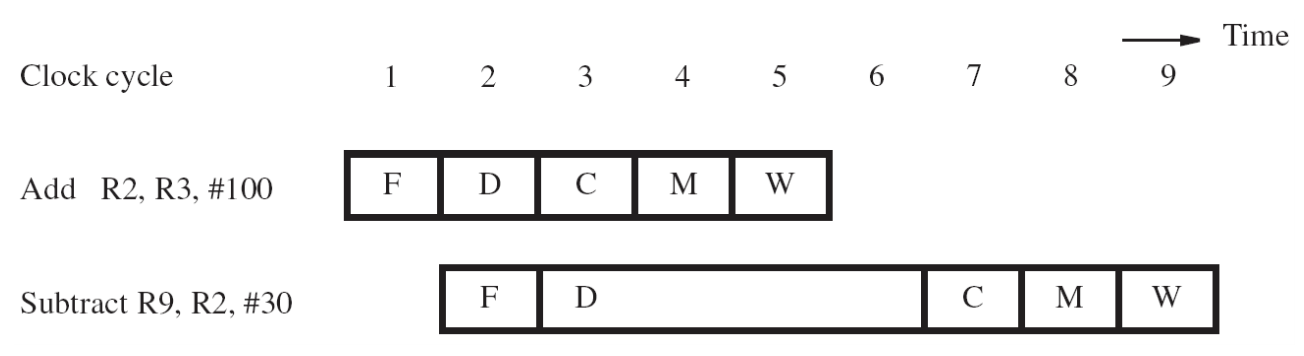
\includegraphics[width=0.8\textwidth]{pipeline/nop.png}
    \item Operand Forwarding: The result of the computation is actually determined in the compute stage, and can be simply forwarded by connecting a wire between RZ and RA/RB. \\
    This allows to handle the hazard without stalling the pipeline\\
    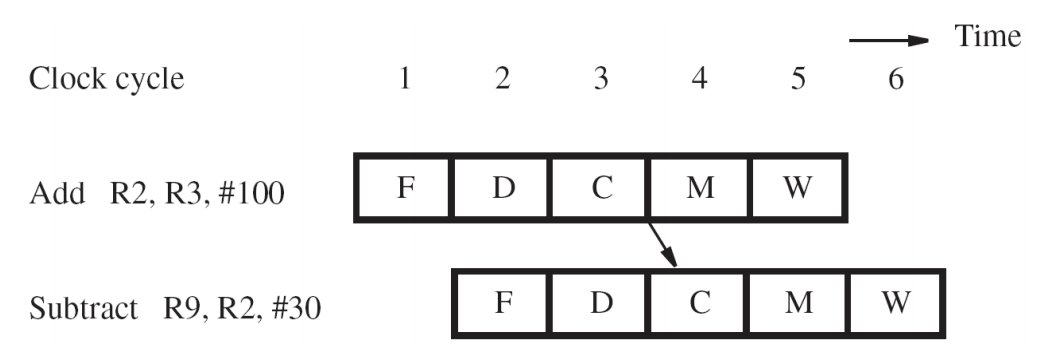
\includegraphics[width=0.6\textwidth]{pipeline/op_forwarding.png}\\
    Although connecting wires is easy, this also expands the logic of our multiplexers at teh register stage, where they now have to choose between the register file and the new RZ [among other for RB]
\end{enumerate}
Memory Stalls still exist, even when there is a cache hit, and must be accounted for.
Cache hit resolves in one cycle, i.e you must wait one cycle at the least. If there is a cache miss then you must wait longer.\\
To solve this:
\begin{enumerate}
    \item Stall until MFC [have to regardless of cache hit/miss]
    \item Forward the result from RY to ALU inputs
\end{enumerate}
\newpage
\subsubsection{Branch Conditions}
\begin{itemize}
    \item \textbf{Unconditional Branch Delays}:
    \begin{itemize}
        \item Branch instruction identified at Decode stage, and target address determined at Compute Stage.
        \item This causes 2 instructions to be fetched, and one of them to be decoded. They must be discarded i.e. 2 cycle penalty
        \item \textit{Fast Branch:} To solve this, just insert another adder inside the decoder to compute the target address i.e. you are now at a one cycle penalty
    \end{itemize}
    \item \textbf{Conditional Branches}: Need to evaluate a condition as well now
    \begin{itemize}
        \item Adder still in decode stage for target address
        \item But comparison still in Execute Stage i.e. still the 2 cycle penalty
        \item Add comparator to decode stage i.e. return to 1 cycle penalty
    \end{itemize}
\end{itemize}
\textbf{Branch Delay Slot}: The instruction right after the branch is the one that is discarded if the branch is taken. This location is called the branch delay slot. We can make effective use of this slot to avoid discarding it. This can be done by re-ordering the instructions to get a non-dependent instruction below the branch the condition from above. This way the instruction fetched after the branch is decoded is always correct, regardless of the branch decision. This can only be done by the compiler, and is not always possible and is called \textit{delayed branching}. If a useful instruction is inserted then the delay is zero, otherwise a NOP causes a delay of 1.\\

\textbf{9.0.2.1 Branch Prediction}\\
\begin{enumerate}
    \item \underline{Static Branch Prediction}: Assume that branch will always not be taken [penalty discovered in decode stage, and predicted accuracy should be 50\%] Accuracy is actually lower than 50 this way, because useful programs have loops, and we can improve accuracy by imposing a condition that if it's a backward branch it'll generally be taken, and a forward branch wont be [the sign of the offset is enough].
    \item \underline{Dynamic Branch prediction}
    \begin{enumerate}
        \item
        \begin{minipage}{0.6\textwidth}
         \textbf{2-state algorithm}:  likely taken (LT) or likely not taken (LNT). Basically assume that the branch will go the same way it went last time, and update state if it doesn't. This prediction, might be changing it's predictions too fast. (2 nested loops, one longer 100, one just 3)
        \end{minipage} \hfill
        \begin{minipage}{0.35\textwidth}
        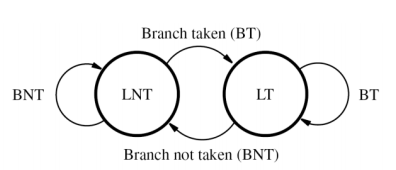
\includegraphics[width=0.8\textwidth]{pipeline/2state.png}
        \end{minipage}
        \item
        \begin{minipage}{0.60\textwidth}
         \textbf{4-state algorithm}:  : strongly taken (ST), likely taken (LT), strongly not taken (SNT), likely not taken (LNT)
        \end{minipage} \hfill
        \begin{minipage}{0.35\textwidth}
        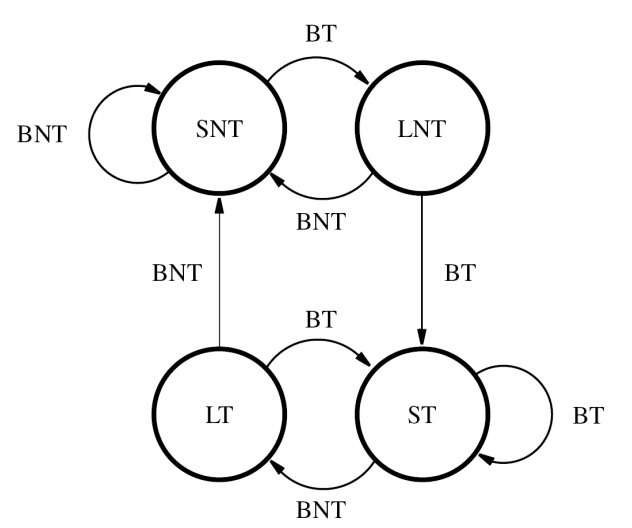
\includegraphics[width=0.8\textwidth]{pipeline/4state.png}
        \end{minipage}
        \\
    \end{enumerate}
\end{enumerate}
\textbf{9.0.2.1 Branch Target Buffer}\\
A Branch Target Buffer (BTB) is a buffer that stores a mapping from PC of branch instructions to their computed target address based on earlier calculations, also stores the branch prediction algorithm bits.\\
If we now move predictor and BTB to the fetch stage, and comparator to decode stage then:
\begin{enumerate}
    \item Cycle 1: use branch instruction address lookup, and then use the bits for prediction
    \item Cycle 2: Fetch next instruction using the prediction
    \item Cycle 3: If incorrect prediction, correct mistake in Decode stage and fetch the correct next instruction
\end{enumerate}
\newpage
\subsection{Performance Evaluations}
\begin{itemize}
    \item T: execution time (seconds/program)
    \item N: dynamic instruction count (instructions/program)
    \item S(CPI): average number of clock cycles to fetch and execute one instruction (cycles/instruction)
    \item R: clock rate (cycles/second)
\end{itemize}
For Non-pipelined:
    $$T = N \times S \times \frac{1}{R}$$
Throughput(P):
    $$P_{np} = \frac{R}{S}\;\;\; [S = 5\;\text{for non-pipelined};\; S = 1\;\text{for pipelined, ideal case i.e. no stalls}]$$
If we account for stalls:
$$P_p = \frac{R}{1 + \delta_{stall}} = \frac{R}{1 + \delta_{load} + \delta_{branch}}$$
\end{document}
